\section{Neural Operators}
\label{sec:neuraloperators}
The universal approximation theorem~\cite{universalT} says that a neural network can approximate an arbitrary continuous function. This fact is exploited widely in the current deep learning research in computer vision, natural language procession, etc. Another important corollary from the universal approximation theorem states that a neural network can also approximate any non-linear continuous functional or operator.

Recently, a new series of works~\cite{deeponet, bhattacharya21, nelsen21, Li20} explore the idea to create a neural operator for solving PDEs. 

Neural operator learns to parameterize a mapping between function spaces instead of learning a mapping between finite-dimensional Euclidean spaces as the classical neural networks do. For PDEs the neural operator learns a mapping between functional parameters to the solutions. This has many advantages compared to classical neural network approaches discussed in \cref{sec:tga}. Neural operator is mesh-independent, since it can transfer the solutions between meshes and used for different discretization. Once neural operator learned, it can be applied to different instances in the whole family of PDE. Furthermore, neural operator does not require the underlying PDE, but only data. 

The recent works can be classified into two categories: approaches that use Euclidean function spaces and those that use Fourier function spaces. 

\subsection{Euclidean Space Operator}
Most of recent works \cite{deeponet, bhattacharya21, nelsen21} focus on defining operators in Euclidean space. Lu et al.~\cite{deeponet} propose a DeepONet --- the first work in this direction. 

This network approximates both linear and non-linear operators from a restricted amount of data, instead of approximating functions. This inputs infinite dimensional functions and outputs other functions but in output space. As shown in \cref{fig:deeponet}, DeepONet comprises two parts: branch and trunk nets. Branch net encodes the discrete input functions at fixed sensors. Trunk net encodes the domain of the output functions. The theoretically proposed architecture is Stacked DeepONet, where branch net is executed $p$ times. In practice, the hyperparameter $p$ is high. In order to reduce computational costs, all branch networks are merged into single branch network.

The proposed method was evaluated on Gravity Pendulum ODE and Diffusion-reaction system. This shows better generalization compared to classical numerical and neural networks approaches. In future works the Li et al. intend to investigate the theoretical network size needed for the neural operator and its connection to generalization error. Moreover, other types of neural network architectures such as CNN, RNN and Transformers can be employed. 

\begin{figure}
	\centering
	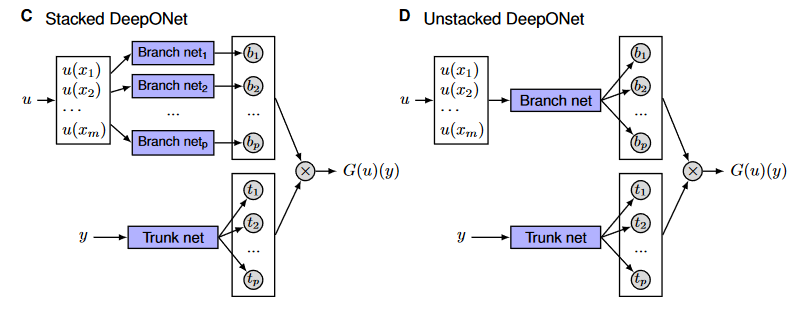
\includegraphics[width=12cm]{figures/deeponet.png}
	\caption{DeepONet comprises two parts: branch net for encoding input functions and trunk net for encoding locations for the output functions~\cite{deeponet}.}
	\label{fig:deeponet}
\end{figure}  

\subsection{Fourier Space Operator}
Differentiation in Euclidean is equivalent to multiplication in Fourier space\cite{diffequimult}. Some hybrid approaches of spectral methods and neural networks exploit this fact for solving PDEs~\cite{fan19, jiang20}. This enhances performance and precision of results, since Fourier space is more suitable for many types of PDEs~\cite{fan19}. Based on these methods, Li et al.~\cite{Li20} introduce a novel fully neural net based Fourier Neural Operator. 

This method was applied to model turbulent flow in 2D, in order to predict how initial vorticity (a curl of velocity that determines the rotational flow in the region) evolves over time. 

\subsubsection{Formal Problem Setting}
In traditional neural net solvers, we input data points with spatial and temporal coordinates $(x, y, t)$, execute the model and receive the solutions as changed with time other data points. In this approach, we input functions $a$ and receive functions $u$ of form mapping $a, u: x, y, t \mapsto vorticity$. Therefore, to solve the PDE we need to determine an operator $G_{\theta}$ with model parameters $\theta$ for input $\mathcal{A}$ and output $\mathcal{U}$ function spaces.
\begin{equation}
G_{\theta}: \mathcal{A} \rightarrow \mathcal{U}, \quad \theta \in \Theta
    \label{eq:fno}
\end{equation}

Due to using function spaces instead of data points, we do not sample on particular resolution. Thus, once functions are learned, any solution resolution is possible. 

\subsubsection{Method}
\label{fno:method}
The pipeline is shown in \cref{fig:fno}(a) and contains two main phases: up- ($P$) and down-projection ($Q$) at the beginning and end, and Fourier Neural Operator (FNO). Up-projection transforms initial state $a(x)$ into latent space. This is implemented with Conv$1\times1$ layer that takes an input tensor described by the sequence of initial timestamps (usually $t=0,...,10$). Afterwards, series of Fourier layers are executed. Finally, down-projection transforms the resulting tensor into output space. The output tensor $u(x)$ contains a sequence of predictions for many timestamps at once (usually $t=11,...,50$). FNO is shown in \cref{fig:fno}(b) and described with \cref{eq:fno1}:

\begin{equation}
v_{t+1}(x):=\sigma\left(W v_{t}(x)+\left(\mathcal{K}(a ; \phi) v_{t}\right)(x)\right)
\label{eq:fno1}
\end{equation}

where $\sigma$ is a non-linearity, $W$ is a weight matrix and $\mathcal{K}$ is a Kernel integral operator that is theoretically described with \cref{eq:fno2}:

\begin{equation}
\left(\mathcal{K}(a ; \phi) v_{t}\right)(x):=\int_{D} \kappa(x, y, a(x), a(y) ; \phi) v_{t}(y) \mathrm{d} y
\label{eq:fno2}
\end{equation}

However, the calculation of $\mathcal{K}$ causes a large computational overhead and is not possible in practice. Lu et al. propose many engineering decisions that simplifies the calculation of $\mathcal{K}$. The main idea is transformation into Fourier space $\mathcal{F}$ where we can use a plain multiplication $R$ instead of calculating convolving integral and back transformation $\mathcal{F}^{-1}$ at the end. This results in \cref{eq:fno3}:

\begin{equation}
\left(\mathcal{K}(\phi) v_{t}\right)(x)=\mathcal{F}^{-1}\left(R_{\phi} \cdot\left(\mathcal{F} v_{t}\right)\right)(x)
\label{eq:fno3}
\end{equation}

\begin{figure}
	\centering
	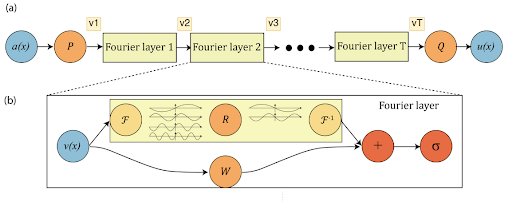
\includegraphics[width=12cm]{figures/fno.png}
	\caption{(a) Pipeline proposed by Li et al.~\cite{Li20} contains two main phases: up- ($P$) and down-projection ($Q$) and Fourier Layers. (b) Fourier Layer contains Fourier forward ($\mathcal{F}$) and back ($\mathcal{F}^{-1}$) transformation and linear multiplication ($R$) equivalent to convolution in Euclidean space.}
	\label{fig:fno}
\end{figure}  

\subsubsection{Results}
The proposed method was evaluated on Burgers, Darcy Flow and Navier--Stokes PDEs. This outperformed all existing learning-based methods in both accuracy and computation time. This is the first method that achieved zero-shot super-resolution for modelling turbulent flows. 

Fourier Neural Operator was mainly applied to modelling turbulent flows, where Fourier spaces were used earlier as a natural approach for this type of problems. Therefore, it remains under discussion, whether FNO can be applied to other PDEs.

Other limitations are related to the Method in \cref{fno:method}. First, the input consists of ten timestamps that have to be computed by either a numerical method or another ML technique. Second, it remains uninvestigated if the super-resolution is bounded and whether the output prediction can be extended to more timestamps at once, i.e. from predefined $t=11,...,50$ to e.g. $t=11,...,200$ or more.



